\documentclass[notitlepage]{article}
\usepackage{graphicx}
\usepackage{bmpsize}
\graphicspath{ {img/} }
\usepackage{courier}
\usepackage{times}
\usepackage[T1]{fontenc}
\usepackage{textcomp}
\usepackage{fullpage}
\usepackage{hhline}
\usepackage{tabular x}
\usepackage{mdframed}
\usepackage{enumerate}
\usepackage{titlesec}
\usepackage{hyperref}
\usepackage[clock]{ifsym}
\newcommand{\sectionbreak}{\clearpage}
\newcommand{\infosign}{\fontencoding{U}\fontfamily{futs}\huge\selectfont\char 116\relax}
\newcommand{\warningsign}{\fontencoding{U}\fontfamily{futs}\Large\selectfont\char 66\relax}
\newcommand{\dangersign}{\fontencoding{U}\fontfamily{futs}\huge\selectfont\char 76\relax}
\newmdenv[linecolor=black,skipabove=\topsep,skipbelow=\topsep,
leftmargin=0pt,rightmargin=0pt,
innerleftmargin=5pt,innerrightmargin=5pt]{infobox}
\makeatletter
\newcommand*{\toccontents}{\@starttoc{toc}}
\makeatother

\begin{document}

\title{\huge{\texttt{ratload}\\ Installation and Use}}
\author{
  Jacob Hladky\\
  California Polytechnic State University\\
  San Luis Obispo, CA\\
  \texttt{jhladky@calpoly.edu}
}
\date{\today}
\maketitle

\toccontents

\pagenumbering{arabic}

\section{Introduction}
The ratload system consists of two separate components: a computer program and a set of VHDL modules. This guide will detail how to install, configure and run both. It is necesssary to follow the instructions in both \emph{Integration} sections, and then either of the \emph{Installation} sections, depending on the target operating system.

\subsection{Requirements}
If you have a Nexys 2 board --- You will need a serial cable. If your computer does not have a serial port, then you will need a USB-to-serial adapter. Here's an example: \url{http://amzn.com/B0007T27H8}. Any adapter will do as long as you have the right drivers for it.\\
If you have a Nexys 3 board --- No serial cable is required, as an onboard FTDI chip provides serial emulation.\\\\
Do not integrate ratload into your RAT CPU until all the major components of the CPU are in place, and you have a good understanding of how they fit together. Understanding how the RAT architecture handles I/O and interrupts will make integration much easier.

\subsection{Project Manifest}
The following is a listing of each file in the \texttt{ratload} system and a brief description of the file's contents and purpose.
\begin{itemize}
\item \texttt{README.pdf} This guide.
\item \texttt{vhdl/RS232RefComp.vhd} UART VHDL module. Required for communication with host computer.
\item \texttt{vhdl/ascii\_to\_int.vhd} VHDL module to convert ASCII-encoded hexidecimal numbers into binary.
\item \texttt{vhdl/prog\_rom.vhd} Replacement prog\_rom module for the RAT CPU.
\item \texttt{vhdl/interceptor.vhd} VHDL module related to the internal operation of the prog\_rom.
\item \texttt{vhdl/prog\_ram.vhd} VHDL module related to the internal operation of the prog\_rom.
\item \texttt{vhdl/real\_prog\_rom.vhd} VHDL module related to the internal operation of the prog\_rom.
\item \texttt{vhdl/serial\_test.vhd} A special prog\_rom module used to test the functionality of the UART.
\item \texttt{asm/serial\_test.asm} Assembly source of the serial\_test VHDL module.
\item \texttt{asm/ratload.asm} Assembly source for the \texttt{ratload} system.
\item \texttt{bin/ratload\_win/} Windows graphical version of the ratload program. The files in this directory are all in support of the Windows ratload program and will not be described individually.
\item \texttt{bin/ratload\_win.exe} Windows command-line version of the ratload program.
\item \texttt{bin/ratload\_nix} Linux command-line version of the ratload program. 
\item \texttt{bin/ratload\_osx} OS X command-line version of the ratload program.
\end{itemize}
Please note there is no graphical ratload program for Linux and OS X.

\begin{infobox}
  {\infosign} The binaries for Linux and OS X may not work for you! (Windows users can disregard this message) Your best bet if you are using a one of these OSes is to compile ratload from source. Instructions for building ratload from source are available in Section~\ref{sec:source_build}.
\end{infobox}

\subsection{Bug Reporting}
All programs have bugs. \texttt{ratload} is beta software and is no exception. If you encounter a bug in either the ratload or the winRATLoad program, please contact the author. It is also possible (albeit significantly less likely) that you find a bug in the project VHDL modules. If you do please verify the bug via simulation and report it immediately so it can be fixed.\\\\
Since you are writing the mechanics of the CPU itself, it is possible for very odd bugs to happen, and for those bugs to interact with \texttt{ratload} in bizarre ways\ldots However \texttt{ratload} has been thoroughly tested and is free of any major bugs.

\subsection{Contact}
If you have any questions about the project itself, or suggestions for improvement for this guide, please contact the author at jhladky@calpoly.edu. This project licensed under the MIT license and the complete source code -- including the \LaTeX ~source for this guide -- is available at \url{http://www.github.com/jhladky/ratload}.


\section{Adding the UART}
Before you can use \texttt{ratload}, you have to add a UART module to your CPU, which is required to communicate with the host computer. Adding the UART is similar to other I/O devices you have encountered such as the 7-segment display driver and the VGA buffer.

\begin{infobox}
  {\infosign} UART stands for ``Universal Asynchronous Receiver-Transmitter'', which you may recognize as another name for a serial port. The UART can be used outside of the \texttt{ratload} project as well. Consider using a UART in your own final project!
\end{infobox}

\subsection{Integration on to RAT CPU}
This section will cover adding the UART module to the RAT CPU and hooking up all the pins to the right places. The UART module is provided by Digilent and is used unmodified here.
\begin {enumerate}
\item In the Xilinx ISE Environment, go to \textbf{Project \textgreater Add Copy of Source}. Navigate to the \texttt{ratload} project directory (where this README is located), and then to the ``vhd'' folder. Select the ``RS232RefComp.vhd'' and ``ascii\_to\_int.vhd'' files and click \textbf{Open}. Another dialog box will pop up confirming you want to add these files. Click \textbf{OK}.

\item In the rat\_wrapper.ucf file (your title may differ slightly), add the following NETs if you have a Nexys 2 board:\\
\centerline{\texttt{NET "TXD" LOC = P9;}}\\
\centerline{\texttt{NET "RXD" LOC = U6;}}\\
If you have a Nexys 3 board, then add these lines instead:\\
\centerline{\texttt{NET "TXD" LOC = XX;}}\\
\centerline{\texttt{NET "RXD" LOC = XX;}}

\item In the architecture section of the top-level rat\_wrapper module, add the following two lines to the entity declaration:\\
\centerline{\texttt{RXD : ~in STD\_LOGIC;}}\\
\centerline{\texttt{TXD : out STD\_LOGIC;}}

\item In the same file, add the following component declarations:
\begin{verbatim}
component RS232RefComp
   Port(
      RXD      : in     STD_LOGIC;
      RST      : in     STD_LOGIC := '0';
      CLK      : in     STD_LOGIC;
      DBIN     : in     STD_LOGIC_VECTOR(7 downto 0);
      RD, WR   : in     STD_LOGIC;
      RDA      : inout  STD_LOGIC;
      TBE      : inout  STD_LOGIC := '1';
      TXD      : out    STD_LOGIC := '1';
      DBOUT    : out    STD_LOGIC_VECTOR(7 downto 0);
      PE, FE   : out    STD_LOGIC;
      OE       : out    STD_LOGIC);
end component;

component ascii_to_int
   Port(
      ascii_in : in     STD_LOGIC_VECTOR(7 downto 0);
      int_out  : out    STD_LOGIC_VECTOR(7 downto 0));
end component;
\end{verbatim}

\item In the same section, add the following signals:
\begin{verbatim}
signal s_d_avail      : STD_LOGIC;
signal s_d_sent       : STD_LOGIC;
signal s_d_strb       : STD_LOGIC;
signal s_d_conf       : STD_LOGIC;
signal s_db_from_rat  : STD_LOGIC_VECTOR(7 downto 0);
signal s_db_to_conv   : STD_LOGIC_VECTOR(7 downto 0);
signal s_db_to_rat    : STD_LOGIC_VECTOR(7 downto 0);
\end{verbatim}

\item Add the following port map for the ascii\_to\_int module:
\begin{verbatim}
CONV: ASCII_TO_INT port map(
   ASCII_IN => S_DB_TO_CONV,
   INT_OUT  => S_DB_TO_RAT);
\end{verbatim}
Data sent over the UART will be ASCII encoded, but we want it to be in hex, so we convert it as soon as it gets out of the UART module. The \texttt{S\_DB\_TO\_CONV} signal receives an ASCII-encoded byte from the UART, and the \texttt{S\_DB\_TO\_RAT} signal has the output in binary.

\item Add the \texttt{S\_DB\_TO\_RAT} signal to whatever method you use to get intputs into the RAT. For example, if you have a  separate input module, then send the signal into that module. If you manage your I/O in the rat\_wrapper module, then add an \texttt{elsif} block. The \texttt{PORT\_ID} for \textbf{input} from the UART is \textbf{0x0F}.

\item Add the following port map for the RS232RefComp module:
\begin{verbatim}
UART: RS232REFCOMP port map(
   RXD     => RXD,
   RST     => RST,
   CLK     => CLK,
   DBIN    => S_DB_FROM_RAT,
   RD      => S_D_CONF,
   WR      => S_D_STRB,
   RDA     => S_D_AVAIL
   TBE     => S_D_SENT,
   TXD     => TXD,
   DBOUT   => S_DB_TO_CONV,
   FE      => open,
   PE      => open,
   OE      => open);
\end{verbatim}
The following is a line-by-line breakdown of the port map:
\begin{itemize}
\item \texttt{RXD}: Receive port for the UART. Serial data goes into the physical UART on the Nexys board and then into this module.
\item \texttt{RST}: Reset for the UART. Hook it up to the RAT's global reset. \textbf{The name of your reset pin may be different!}
\item \texttt{CLK}: Clock for the UART. Hook it up to yer clock. \showclock {9}{0}
\item \texttt{S\_DB\_FROM\_RAT}: Send bus.
\item \texttt{S\_D\_CONF}: Read strobe. We take it high to confirm that data has been received.
\item \texttt{S\_D\_STRB}: Write strobe. We take it high to indicate we have data on \texttt{S\_DB\_FROM\_RAT} to send.
\item \texttt{S\_D\_AVAIL}: Indicates data is available to be read.
\item \texttt{S\_D\_SEND}: Indicates data has been successfully sent.
\item \texttt{TXD}: Transmit port for the UART, similar to the receive port.
\item \texttt{DBOUT}: Receive bus
\item \texttt{FE, PE, OE}: Error pins. ``Frame Error'', ``Parity Error'', and ``Output Error'', respectively. We're not concerned with checking for data errors so we leave these pins open.
\end{itemize}

\item Modify your outputs process (or module) to send data to the UART.
\begin{infobox}
  {\warningsign} \textbf{THIS IS A CRITICAL STEP!} I/O devices like the UART require more than just a simple data bus for proper operation. In the previous step you hooked-up several control signals to the UART modue, now you have to hook-up the other end! For convenience sake we will have the output process control these signals, and to make it really easy, an example output process is reproduced here.
\end{infobox}
You may need to adapt some of the signal names to fit your conventions. \textbf{Make sure to do so without changing the UART signals!}
\begin{verbatim}
CONSTANT UART_OUT_ID   : STD_LOGIC_VECTOR(7 downto 0) := x"0E";

outputs: process(CLK) begin
   if (rising_edge(CLK)) then
      s_d_strb <= '0';
      s_d_conf <= '0';
      if (S_IO_OE = '1') then
         if (s_port_id = LEDS_ID) then
            LEDS <= s_output_port;
         elsif (s_port_id = UART_OUT_ID) then
            s_db_from_rat <= s_output_port;
            s_d_strb <= '1';
            s_d_conf <= '1';
         end if;
      end if;
   end if;
end process outputs;
\end{verbatim}

\item Make sure that you can successfully synthesize your RAT\_wrapper with the UART integrated. This is the last step in integrating the UART.
\begin{infobox}
  \textbf{{\warningsign}} You will receive the following warning about a latch:\\
    \centerline{\texttt{Found 1-bit latch for signal \textless TBE\textgreater. Latches may be \ldots}}\\
    This is a result of a flaw in the Digilent Romania provided UART module. It is safe to ignore. Any other latch, however, is not the result of this flaw and must be fixed!
\end{infobox}
\end{enumerate}

\subsection{Verification}
This section covers a quick test of the UART module you just integrated into your RAT CPU. If the test in this section is not 100\% successful \textbf{DO NOT CONTINUE}. Go back and double check that you have integrated the UART properly. If the UART continues not to work, go to the ``Troubleshooting'' section. \textbf{\texttt{RATLOAD} WILL NOT WORK UNLESS YOUR UART BEHAVES EXACTLY AS EXPECTED!}

\begin{enumerate}
\item Replace your current prog\_rom module with the prog\_rom module in the ``serial\_test.vhd'' file, in the ``vhdl'' folder. Then program your Nexys board with the new bit file.
\item Hook up the serial cable to the Nexys and the host computer. This step involves running the ratload program. For more information about installing and running the ratload program see the ``Installation'' and ``Use'' sections.
  \begin{enumerate}[a.]
  \item \textbf{Graphical version (Windows only) ---} Select the proper serial device from the dropdown menu. Then go to \textbf{File \textgreater Run Serial Test}. The program will then attempt to communicate with the Nexys board via the serial cable. If the results window says ``PASS'', then move on to the next section. If it says anything else, then go back and make sure you followed the integration instructions properly.

  \item \textbf{Command-line version ---} Run ratload in test mode like so:
\begin{verbatim}
ratload -d /dev/<serial device> --test
\end{verbatim}
If the program prints out ``PASS'', then you can skip the ``Troubleshooting'' section. If it says anything else, then go back and make sure you followed the integration instructions properly.
  \end{enumerate}
\end{enumerate}

\subsection{Troubleshooting}
The easiest way to troubleshoot the UART module is to break out an actual serial console and see what it's sending to the computer. So that's what we're going to do. You will need to know what your serial device is called on your computer. To do so see Section~\ref{sec:serial_id}.
\subsubsection{Obtaining a serial console}
\begin{itemize}
\item \textbf{Windows users --- } A good serial console for Windows is putty. Download putty from here:\\
  \centerline{\url{http://www.chiark.greenend.org.uk/~sgtatham/putty/download.html}}
\item \textbf{Linux users --- } Install minicom with your package manager. If you are using a debian-based disto that looks like: \texttt{sudo apt-get install minicom}.
\item \textbf{OS X users --- } Install minicom with homebrew, macports, whatever. That will look like: \texttt{brew install minicom}.
\end{itemize}

\subsubsection{Configuring the proper serial console settings}
\begin{itemize}
\item \textbf{Windows users --- }
  Run putty. From the \textbf{Connection Type} options, select the \textbf{Serial} radio button. Enter the COM port of your serial device in the \textbf{Serial Line} box. Before you can connect on the serial line you need to make sure it has the correct settings. Make your putty settings look like they do in Figure~\ref{fig:putty}. Remember that your COM port may differ. After you have entered the correct settings click \textbf{Open}.
\begin{figure}[ht!]
  \centering
  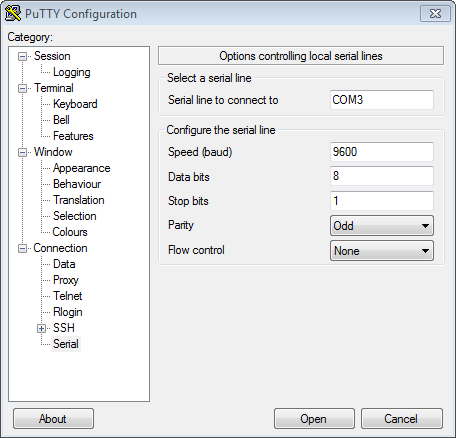
\includegraphics[width=0.5\textwidth]{fig0.png}
  \caption{The correct settings to use with Putty}
  \label{fig:putty}
\end{figure}
\item \textbf{Linux and OS X users --- } Start minicom from the terminal in config mode by using the \texttt{-s} flag, like so: \texttt{minicom -s}. Use your keyboard to navigate the configuration menu that pops up. Select the \textbf{Serial Port Setup} option. Make your minicom settings look like they do in Figure~\ref{fig:minicom}. Remember that your serial device and ``Lockfile Location'' may differ (you can ignore ``Lockfile Location'', actually). After you gave entered the correct settings hit escape until minicom dumps you out to the serial console window.
\begin{figure}[ht!]
  \centering
  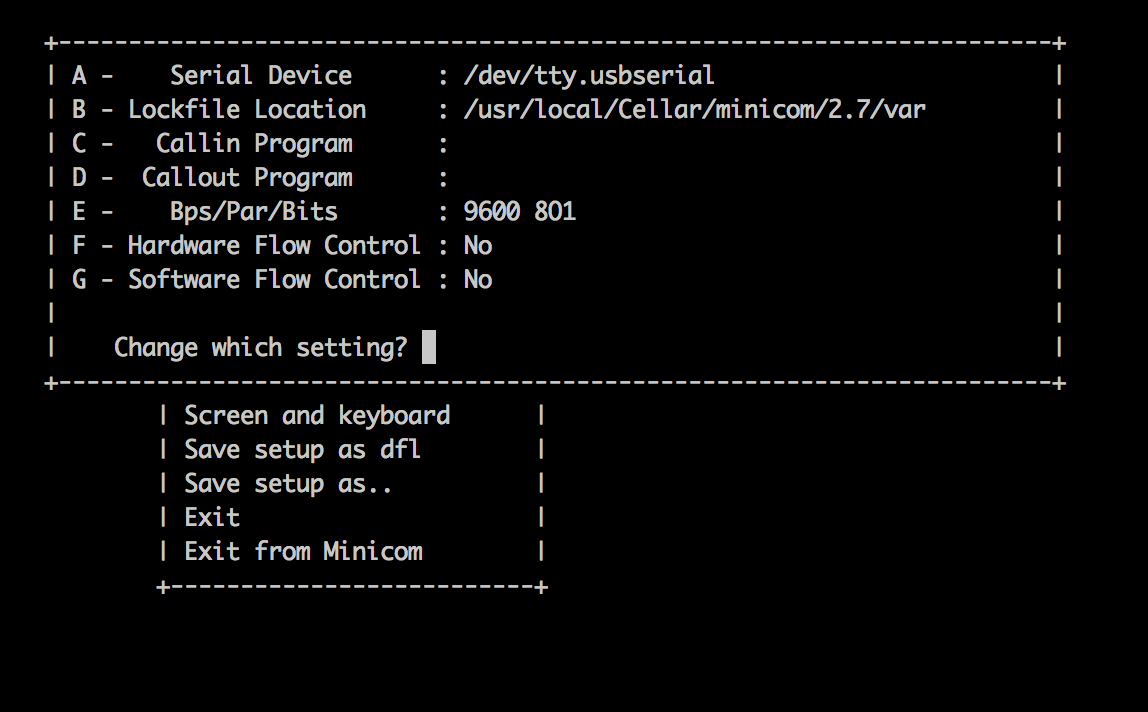
\includegraphics[width=0.5\textwidth]{fig1.png}
  \caption{The correct settings to use with minicom}
  \label{fig:minicom}
\end{figure}
\end{itemize}

\subsubsection{Using the serial console to troubleshoot the UART}
Once you have your serial console up and running flash your Nexys board with your bit file that has the serial test program on it. (Make sure you've connected the Nexys board to your computer with the serial cable).

\section{Adding the New Prog\_Rom module}
Once you have added the UART and verified that it is functioning correctly, the remaining steps are simple.
\begin{enumerate}
\item Go to \textbf{Project \textgreater Add Copy of Source}. Navigate to the \texttt{ratload} directory again and then to the same ``vhdl'' folder. Select the ``prog\_rom.vhd'', ``prog\_ram.vhd'', ``real\_prog\_rom.vhd'', and ``interceptor.vhd'' files and click \textbf{Open}. Another dialog box will pop up confirming you want to add these files. Click \textbf{OK}.

\begin{infobox}
  {\warningsign} This is a destructive action and will overwrite any files already in your project directory that have a name identical to the files being added e.g. any existing prog\_rom.vhd file will be overwritten by the \texttt{ratload} prog\_rom.vhd file.
\end{infobox}

\item In the architecture section of the rat\_cpu module, edit the componet declaration for the prog\_rom module. Add the following line:\\
\centerline{\texttt{TRISTATE\_IN : in STD\_LOGIC\_VECTOR(7 downto 0)}}

\item In the same file, edit the port map decaration for the prog\_rom module. Map the signal for the RAT CPU's tristate bus into to the prog\_rom module's tristate bus. The RAT CPU's ``tristate\_bus'' may be called the ``MULTI\_BUS'' in your CPU. (Regardless of its name, this is the bux that connects the ALU, the program counter, the scratch pad, and others.) That line will look similar to this:\\
  \centerline{\texttt{tristate\_in =\textgreater ~tristate\_bus\_sig(7 downto 0),}}

\item Synthesize and generate a bit file for your newly integrated system. That's it! \texttt{Ratload} should work on your CPU now. The next sections cover installing and using the ratload program.
\end{enumerate}

\section{Installing the Ratload Program}
Installation is really easy. For all platforms the command-line ratload binary is self-contained. Installation consists of copying the program to a location convenient to you. Make sure to choose the binary corresponding to your platform. Linux users need ``ratload\_nix'', OS X users need ``ratload\_osx'', and Windows users need ``ratload\_win.exe''. Instructions for using the grapical version of ratload (Windows only) and for building from source and included below.

\subsection{Graphical ratload (Windows only)}
The graphical version of the ratload program is located in the folder ``ratload\_win''. Copy the entire folder somewhere useful to you. The graphical program will not work without the container folder. There is no other installation step.

\subsection{Building from source}
\label{sec:source_build}
The Windows versions of ratload contain statically linked binaries and thus are unlikely to malfunction across different versions of Windows. The Linux and OS X versions are not statically linked and if you have problems running them you should compile ratload from source.\\\\
Ratload has no dependencies other than the libc and should build and run on any POSIX-compliant OS. The source is available at \url{http://github.com/jhladky/ratload}, in the \texttt{nix} folder. Clone the repo and build the program with \texttt{make}.\\\\
You must have some sort of build environment set up for this to work. Mac users should have XCode tools installed and get gcc or clang via homebrew/macports/fink, etc. GNU/Linux users should install gcc via their package manager. If you're using a debian based distribution, such as Linux Mint or Ubuntu, then the following will get everything you need:\\
\centerline{\texttt{sudo apt-get install build-essential}}\\\\
If you're using some other distro I'm not going to help you because you know what you're doing. After building the binary, follow the above instructions for your relevant OS.

\section{Use}
\subsection{Identifying your Serial Device}
\label{sec:serial_id}
\begin{itemize}
\item \textbf{Windows users --- } Run the graphical ratload program. The main window of the program contains a dropdown which lists your available serial devices. If you are using a USB-to-serial adapter the easiest way to be totally sure of the correct COM port number is to unplug the adapter and run the graphical ratload program. While the adapter is still unplugged, note the adapters listed. Then plug in the adapter and click \textbf{File > Refresh Serial Devices}. The COM port that appears in the dropdown is the COM port of the adapter.

\item \textbf{Linux and OS X users --- } In GNU/Linux or OS X, list the contents of the \texttt{/dev} folder. In GNU/Linux your serial adapter will be called something similar to ``ttyS0''. In OS X, it will look like ``tty.usb0'' or similar.
\end{itemize}

%% Before you use the ratload program you have to make your serial port is set up. Follow either of the following sections based on which Nexys board version you have.
%% \subsubsection{Nexys 2}
%% If you have a serial port on your computer, congratulations, you are using a computer from the 20th century! Your OS almost certainly already has installed drivers to use this port, so you don't need to do anything else.\\\\
%% If you don't have a serial port, then you need to obtain a USB-to-serial adapter cable. If you're on Windows, the manufacturer of the cable probably provided drivers for you to install along with the cable itself, make sure you install them. If you're using GNU/Linux or OS X, google around to try to find the right driver.\\\\
%% Once you think you've installed the driver then you simply need to verify that the OS can see it. In Windows 7, go to the Start menu and right click Computer, and then click manage. Look for the serial device in the device management section of the console. 
%% \subsubsection{Nexys 3}
%% If you have a serial port on your computer, it doesn't matter, you can't use it! The Nexys 3 doesn't have a physical serial port, but instead emulates one with an FTDI chip. The USB cable you use to power and program the board also functions as a serial cable when it needs to. This means you need to install an FTDI driver. FTDI drivers for OS X and Windows 7 are included in the project folder. Install them and be glad you don't have to deal with USB-to-serial cable drivers!

Up until now, you've probably followed this pattern when developing your assembly language programs:
\begin{enumerate}
\item Run your assembly repeatedly in the ratsim program until it produces a prog\_rom.vhd file and seems to be relatively bug free.
\item Add the new prog\_rom.vhd file to your project, replacing the old one.
\item Resynthesize the entire project and reprogram the bit file onto your Nexys board.
\item Repeat ad infinitum.
\end{enumerate}
The steps you have just followed to integrate the vhd files into your RAT CPU, and to install the ratload program onto your computer, will dramatically change this pattern. From now on you do not need to resynthesize your project when ratsim generates a new prog\_rom.vhd file, nor is it necessary to copy that new file into your project. In fact, \textbf{making any more changes to the prog\_rom.vhd file in your project directory will break \texttt{ratload}}.\\\\
The following is a general overview of the new pattern you need to follow in order to use \texttt{ratload} properly:

\begin{enumerate}
\item Program your Nexys board with the generated bit file.

\item Without disconnecting anything else, connect the Nexys 2 board to your computer via the serial cable. \textbf{If you have a Nexys 3 board, ignore this step.}

\item Start either the winRATLoad or the ratload program, depending on your OS. Select the proper serial device and prog\_rom.vhd file to read.

\item The program will then communicate with the Nexys board and send the prog\_rom.vhd to your RAT CPU via the serial connection. Once the program displays a success message, the serial cable (again, only if you have a Nexys 2) can be disconnected and the board used normally. You can treat the program running on the board like it was synthesized with the system using the previous pattern.

\item To send a new prog\_rom.vhd file you must power cycle the Nexys board (If you programmed your bit file into volatile memory, then you'll need to reprogram it as well.) Then repeat this procedure.
\end{enumerate}

\subsection{Using winRATLoad (Windows)}

\subsection{Using ratload (GNU/Linux or OS X)}
ratload takes exactly two arguments: ``-d'' to specify a serial sevice and ``-f'' to specify a prog\_rom.vhd file to parse. You'll probably have to run it as root in order to access the serial device. The following is an exlpanation of all the errors messages ratload can produce:
\begin{itemize}
\item ``Opening prog\_rom failed'': Ratload could not open your prog\_rom.vhd file. Perhaps it couldn't find it, or it didn't have permission.
\item ``Opening serial device failed'': Ratload could not open the serial device you specified. Perhaps you specified it incorrectly, or ratload does not have permission to access it.
\item ``Invalid prog\_rom.vhd file, exiting.'': Ratload was able to find and open the file you specified, but it couldn't parse it. Ratload expects the prog\_rom.vhd to be structured in a very specific way. Because this file is auto-generated by the ratsim program, this is not a problem. Make sure you are specifying the exact prog\_rom.vhd file that ratsim generates. If you continue to receive this error, try generating the prog\_rom.vhd file again.
\item ``Serial Configuration Failed'': Ratload was able to find and open the device you specified, but when it failed to configure it. It is possible but extremely unlikely that you have a serial device that does not support the proper settings. It is much more like that you specified a valid but incorrect device.
\item ``Error communicating with Nexys2 board.'': Ratload was able to open and parse the file you specified, and was able to open and configure the serial device you specified, but it received no or incorrect data from the Nexys board. Program the ``reference\_rat\_wrapper.bit'' file onto your Nexys board and try to send data to it wih ratload. If that works, then you have misconfigured your RAT CPU, and you need to return to the integration section and make sure you followed those steps correctly. 
\item ``Too many [few] arguments.'': You specified the arguments to ratload incorrectly.
\item ``Option not supported. Only -f and -d supported.'': You specified the arguments to ratload incorrectly.
\end{itemize}
\end{document}
